
\section{Learning about motion}

When the robot pokes an object and acquires its segmentation,
it is straightforward to track how the object moves after impact.
%
Pooling this data over all objects reveals how the movement of the
robot's arm~-- which can approach the object from several directions
-- correlates with the final movement of the object.

But not all objects behave the same way when struck.  
Some objects have a preferred direction of motion~-- for example,
a toy car tends to roll forward along its principal axis,
or a bottle might roll along its side.
%
The robot was made sensitive to differences in object motion
conditioned on object identity (color histogram) and principal axis.
The robot exhibited what it learned in two ways.  It would 
attempt to strike objects so that they would roll.
It also engaged in
simple form of mimicry (see Figure~\ref{fig:mimicked-action}).
If the human companion moved an object in a way that
exploited an ``affordance'' such as rolling, 
the robot would attempt to do the same; if the human moved the
object in an ``unnatural'' way, the robot would attempt to
copy this too.

\ifnote
\begin{figure}[tb]
\begin{center}
%%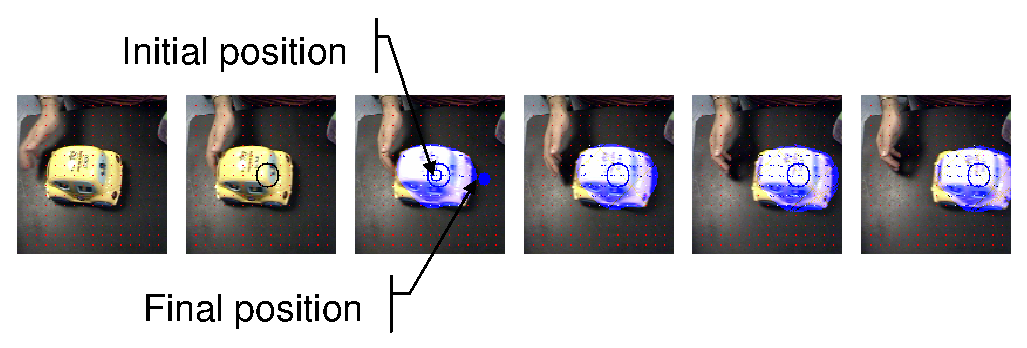
\includegraphics[width=\columnwidth]{observed-action.eps}
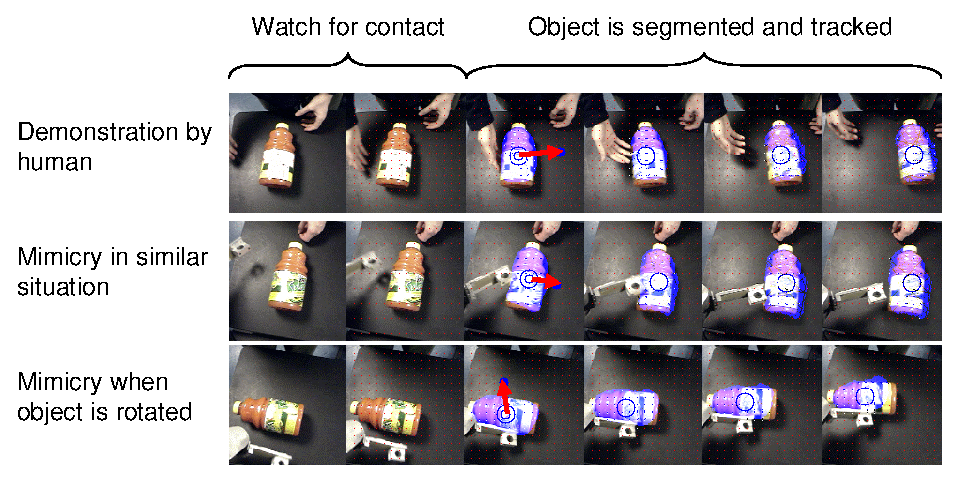
\includegraphics[width=\columnwidth]{fig-mimicry-bottle}
\caption{ 
\label{fig:observed-action}
%
Basic mimicry.  The first step in mimicking an action is to actually
be able to observe it.  The first sequence shows a human demonstration
of a poking operation.  Frames around the moment of contact are shown.
The object, after segmentation, is tracked for 12 frames using a
combination of template matching and optic flow.  The big circles
represent the tracked position of the bottle in successive frames.
The arrow displayed on the frame of contact ($3^{rd}$ from the left)
projects from the position at the time of contact and at the $12^{th}$
frame respectively.
%
In the second sequence, the bottle is presented to the robot in the
same orientation it had in the demonstrated action and the robot
repeats the observed action, a ``side tap''.  In the third sequence,
the car is presented at a different angle.  The appropriate action to
exploit the affordance and make the bottle roll is now a ``back
slap''.
%
}
\end{center}
\end{figure}
\fi

\begin{figure}[tb]
\begin{center}
%%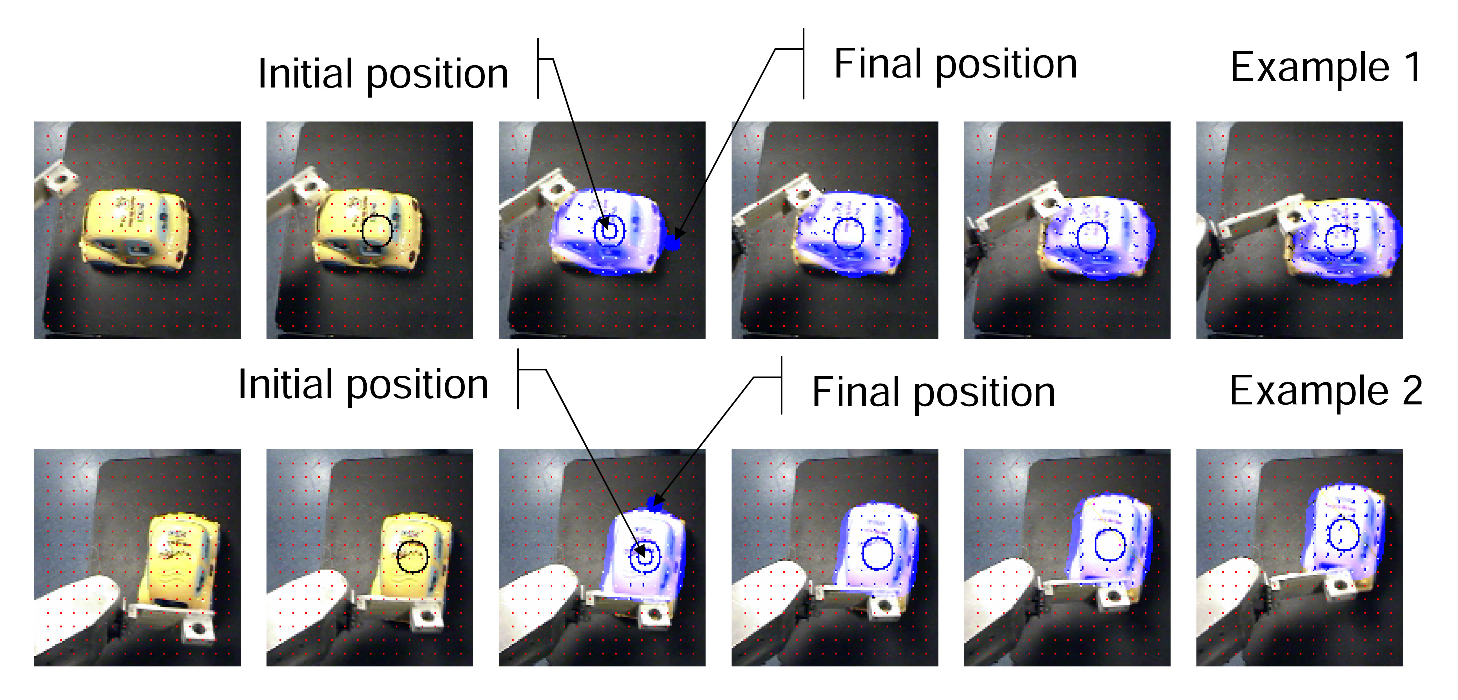
\includegraphics[width=\columnwidth]{mimicked-action.eps}
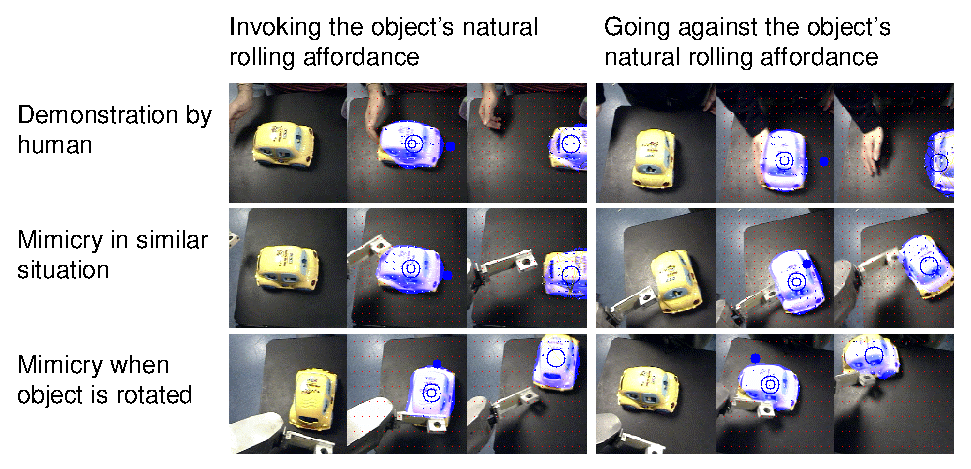
\includegraphics[width=\columnwidth]{fig-mimicry-awkward.eps}
\caption{ 
\label{fig:mimicked-action}
%
%
The sequences on the left show the robot mimicking a human exploiting
a car's rolling ``affordance''.  The sequences on the right show
what happens when the human hits the car in a contrary fashion, going
against its preferred direction of motion.  The robot mimics this 
``unnatural'' action, suppressing its usual behavior of trying to
evoke rolling.
%n extended mimicry example using the toy car.
%The sequences on the left show the robot mimicking a human exploiting
%the car's rolling affordance.  The sequences on the right show
%what happens when the human hits the car in a contrary fashion, going
%against its preferred direction of motion.  The robot mimics this 
%``unnatural'' action, suppressing its usual behavior of trying to
%evoke rolling.
%
}
\end{center}
\end{figure}

